% Idee: Andres Alumets
% Tekst: Andres Alumets

\documentclass[a4paper,11pt]{article}
\usepackage[et]{../../eio}
\usepackage{wrapfig}
\usepackage{tikz}

\begin{document}
\begin{ol}{\eio}{\lv 07.--13.10.2024}{\yle}{}
    \begin{yl}{3}{Neljakandilised saelauad}{vandra}{1 sek / 3 sek}{40 punkti}
        Vändras on maailmakuulus saekaater. Hetkel on neil valmis tehtud $N$ lauda. Selleks, et kliendid saaks laudade kvaliteeti hinnata, laotati need laiali ühe suure ristkülikukujulise ruumi põrandale. Iga laua kohta on teada, et selle ääred on paralleelsed ruumi seintega. Kliendid pole õnnelikud, kui mõni laud teise ära katab. Seega tahab saekaater olla kindel, et ükski laud ei asu ühegi teise peal (puutuda tohivad, sest siis on mõlemad lauad ikka tervenisti nähtavad).

        Kas leiduvad kaks lauda, mis vähemalt osaliselt kattuvad?

        \sis Sisendi esimesel real on laudade arv $N$ ($1 \le N \le 10^5$). Järgmisel $N$ real on igaühel neli täisarvu $X_1, Y_1, X_2, Y_2$ ($0 \le X_1 < X_2 \le 10^9$, $0 \le Y_1 < Y_2 \le 10^9$): ühe laua vasaku alumise ja parema ülemise nurga koordinaadid. Koordinaatide nullpunkt on põranda vasak alumine nurk.

        \val Kui sisendis leiduvad kaks lauda, mis vähemalt osaliselt kattuvad, siis väljastada `\verb/JAH/', muidu väljastada `\verb/EI/'.

        \begin{wrapfigure}[3]{r}{0.4\textwidth}
          \centering
          \vspace{-1cm}
          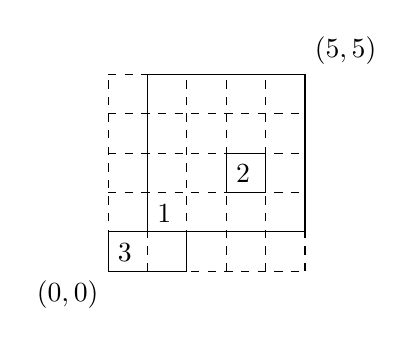
\begin{tikzpicture}[scale=0.50]
            \draw[dashed] (0, 0) node[below left] {$(0, 0)$} grid (5, 5) node[above right] {$(5, 5)$};
            \draw (1, 1) node[above right] {$1$} rectangle (5, 5);
            \draw (3, 2) node[above right] {$2$} rectangle (4, 3);
            \draw (0, 0) node[above right] {$3$} rectangle (2, 1);
          \end{tikzpicture}
        \end{wrapfigure}

        \nde[0]{3cm}{3cm}

        Esimene ja teine laud kattuvad. Kolmas laud küll puutub esimest, kuid kattumist ei ole.

        \nde[1]{3cm}{3cm}
        
        Kuna testis on ainult üks laud, siis mingeid kattumisi olla ei saa.

        \hnd Selles ülesandes on testid jagatud gruppidesse. Iga grupi eest saavad punkte ainult need lahendused, mis läbivad \textbf{kõik} sellesse gruppi kuuluvad testid. Gruppides kehtivad järgnevad lisatingimused:

        \begin{xenum}
            \item ($0$ punkti) Näited.
            \item ($20$ punkti) $N \le 10^3$.
            \item ($10$ punkti) Mistahes kaks lauda kas kattuvad või ei puutu üldse kokku.
            \item ($10$ punkti) Lisapiirangud puuduvad.
        \end{xenum}
    \end{yl}
\end{ol}
\end{document}
